\documentclass[unknownkeysallowed]{beamer}
\mode<presentation>
{
%  \usetheme{AnnArbor}
%  \usetheme{Dresden}
%  \usetheme{Montpellier}
%  \usetheme{Antibes}
%  \usetheme{Frankfurt}
%  \usetheme{PaloAlto}
%  \usetheme{Bergen}
%  \usetheme{Boadilla}
%  \usetheme{Goettingen}
%  \usetheme{Pittsburgh}	%!!
%  \usetheme{Berkeley}
%  \usetheme{Hannover}
%  \usetheme{Rochester}		%!!!
%  \usetheme{Berlin}
%  \usetheme{Ilmenau}
%  \usetheme{Singapore}
  \usetheme{Boadilla}		%viel platz
%  \usetheme{JuanLesPins}
%  \usetheme{Szeged}		%!
%  \usetheme{boxes}
%  \usetheme{Luebeck}
%  \usetheme{Warsaw}
%  \usetheme{Copenhagen}
%  \usetheme{Madrid}
%  \usetheme{Darmstadt}
%  \usetheme{Malmoe}
%  \usetheme{default}
%  \usetheme{JuanLesPins}

%  \usetheme{Marburg}


%\usefonttheme{professionalfonts}
%	default | professionalfonts | serif |
%	structurebold | structureitalicserif |
%	structuresmallcapsserif
%\useinnertheme{rounded}
%	circles | default | inmargin |
%	rectangles | rounded

%  \setbeamercovered{transparent}
  % oder auch nicht
\usecolortheme{rose}


\definecolor{uaf yellow}{cmyk}{0,0.16,1,0} % official UAF yellow
\definecolor{light yellow}{cmyk}{0.01,0,0.16,0}
\definecolor{uaf blue}{cmyk}{1,0.66,0,0.02} % official UAF blue
\definecolor{light blue}{cmyk}{0.22,0.11,0,0}
\definecolor{arsc blue}{HTML}{005496}
\definecolor{arsc red}{HTML}{a20a42}
\definecolor{arsc green}{HTML}{009a82}
\definecolor{light gray}{HTML}{777777}

  %navigation aus, klaut nur platz
  \setbeamertemplate{navigation symbols}{}
% Reset title background to default
%\setbeamertemplate{title page}[default]
\setbeamercolor{title}{bg=}
\setbeamercolor{frametitle}{bg=uaf blue, fg=white}
\setbeamercolor{institute}{fg=white}
\setbeamercolor{date}{fg=white}
\setbeamercolor{block}{bg=}
%\setbeamercolor{title}{fg=black}

% Reset block background to default
%\setbeamertemplate{blocks}[default]
%\setbeamercolor{block title}{bg=}
%\setbeamercolor{block body}{bg=}

\beamertemplatenavigationsymbolsempty  
\setbeamertemplate{blocks}[rounded][shadows=false]

\useinnertheme{circles}

}
\usepackage[latin1]{inputenc}
\usepackage{latexsym}
\usepackage{amsfonts}
%\usepackage{natbib}
\usepackage{fancyhdr}
\usepackage{graphicx}
%\usepackage{subfigure}
% oder was auch immer
\usepackage{grffile}
\usepackage{pgf}
\usepackage{tikz}

\usepackage{listings}

\usepackage{times}
\usepackage[T1]{fontenc}
%\usepackage{appendixnumber}
% Oder was auch immer. Zu beachten ist, das Font und Encoding passen
% m�ssen. Falls T1 nicht funktioniert, kann man versuchen, die Zeile
% mit fontenc zu l�schen.

\hypersetup{
    bookmarks=true,         % show bookmarks bar?
    unicode=false,          % non-Latin characters in Acrobat's bookmarks
    pdftoolbar=true,        % show Acrobat's toolbar?
    pdfmenubar=true,        % show Acrobat's menu?
    pdffitwindow=false,     % window fit to page when opened
    pdfstartview={FitH},    % fits the width of the page to the window
    pdftitle={My title},    % title
    pdfauthor={Author},     % author
    pdfsubject={Subject},   % subject of the document
    pdfcreator={Creator},   % creator of the document
    pdfproducer={Producer}, % producer of the document
    pdfkeywords={keyword1} {key2} {key3}, % list of keywords
    pdfnewwindow=true,      % links in new window
    colorlinks=false,       % false: boxed links; true: colored links
    linkcolor=red,          % color of internal links
    citecolor=green,        % color of links to bibliography
    filecolor=magenta,      % color of file links
    urlcolor=cyan           % color of external links
}

\title[PAG]% (optional, nur bei langen Titeln n�tig)
{GEOS 436 / 636\\
Programming and Automation for Geoscientists\\[20pt]
-- Week 05: Python's NumPy \& Pandas --
}

\author[Grapenthin]% (optional, nur bei vielen Autoren)
{Ronni Grapenthin\\
rgrapenthin@alaska.edu\\
Elvey 413B\\
x7682}
% - Namen m�ssen in derselben Reihenfolge wie im Papier erscheinen.
% - Der \inst{?} Befehl sollte nur verwendet werden, wenn die Autoren
%   unterschiedlichen Instituten angeh�ren.

\institute[UAF] % (optional, aber oft n�tig)
{}
% - Der \inst{?} Befehl sollte nur verwendet werden, wenn die Autoren
%   unterschiedlichen Instituten angeh�ren.
% - Keep it simple, niemand interessiert sich f�r die genau Adresse.

% - Namen m�ssen in derselben Reihenfolge wie im Papier erscheinen.
% - Der \inst{?} Befehl sollte nur verwendet werden, wenn die Autoren
%   unterschiedlichen Instituten angeh�ren.

% - Der \inst{?} Befehl sollte nur verwendet werden, wenn die Autoren
%   unterschiedlichen Instituten angeh�ren.
% - Keep it simple, niemand interessiert sich f�r die genau Adresse.

\date[September 24, 2020] % (optional, sollte der abgek�rzte Konferenzname sein)
{September 24, 2020}

% - Volle oder abgek�rzter Name sind m�glich.
% - Dieser Eintrag ist nicht f�r das Publikum gedacht (das wei�
%   n�mlich, bei welcher Konferenz es ist), sondern f�r Leute, die diese
%   Folien sp�ter lesen.

%\AtBeginSection[]
%{
%  \begin{frame}<beamer>
%    \frametitle{Outline}
%    \tableofcontents[currentsection,currentsubsection]
%  \end{frame}
%}

% Falls Aufz�hlungen immer schrittweise gezeigt werden sollen, kann
% folgendes Kommando benutzt werden:

%\beamerdefaultoverlayspecification{<+->}

%%switch on to have only frame numbers
\setbeamertemplate{footline}[frame number]

\defbeamertemplate*{title page}{customized}[1][]
{
		\begin{tikzpicture}
			\node[text width=\textwidth,
				fill=gray!70, 
				fill opacity=0.75,
				text opacity=1,
				rounded corners = 10pt,
				inner sep=2pt]{
				\begin{center}	
			  \usebeamerfont{title}{\bf \usebeamercolor[fg]{title} \inserttitle}
			  \par
			  \usebeamerfont{subtitle}\insertsubtitle\par
			  \bigskip
			  \usebeamerfont{author}\insertauthor\par
			  \bigskip
			  \usebeamerfont{institute}\insertinstitute\par
			  \bigskip
			  \usebeamerfont{date}\insertdate\par
			  \end{center}
			  };
	\end{tikzpicture}		  
%	\vspace{0.4cm}\usebeamercolor[fg]{titlegraphic}\inserttitlegraphic 
%	\begin{flushright}
%	\vspace{-1.25cm}\includegraphics[width=2cm]{../moore_logo_transp.png}\vspace{5cm}
%	\end{flushright}
}

\begin{document}

\lstset{numbers=left, numberstyle=\tiny, stepnumber=2, basicstyle=\ttfamily, numbersep=5pt, xleftmargin=10pt}

\setbeamertemplate{background}{\includegraphics[width=\paperwidth]{/home/roon/Pictures/rooftop_initial.jpg}}

	\begin{frame}
	\begin{center}
		\titlepage
	\end{center}
	\end{frame}

\setbeamertemplate{background}{}

\begin{frame}
\frametitle{}
	\vspace{2cm}
	\begin{center}
		Key concept in programming and automation: Use existing tools!
	\end{center}
%	\vspace{4cm}
\end{frame}

\begin{frame}
	\frametitle{Advanced Data Types}
	\begin{itemize}
		\item We've dealt with a few basic data types so far: {\tt int, boolean, float, \dots}
		\item You know about more complex data types like lists (arrays), dictionaries in Python
		\item Most of your data are some form of table where measurements (float values) are connected to moments in time or locations in space (other float values)
		\item Even images fall in this category
		\item Have data types that provide efficient storage and operation on such data: Numpy array, Pandas Series \& DataFrame
	\end{itemize}
	
\end{frame}

\begin{frame}
	\frametitle{NumPy}
		\begin{itemize}
			\item ``The fundamental package for scientific computing with Python''
			\item It's a library (or package) that expands the functionality of core-Python
			\item Provides multidimensional array ({\tt ndarray}) object (and efficient storage)
			\item Provides functions that efficiently (read fast) operate on this data type
			\item As opposed to the Python list, dictionary types, data in {\tt ndarray} must be homogeneous, i.e. of the same type
			\item Large infrastructure of Python-based packages use {\tt ndarray} internally, being proficient in its use is necessary to leverage those packages
		\end{itemize}
\end{frame}

\begin{frame}
	\frametitle{NumPy}
		\begin{center}
		NumPy = {\tt ndarray} + functions
		\end{center}
\end{frame}

\begin{frame}
	\frametitle{NumPy Overview}
		\vspace{-0.25cm}
		\begin{center}
			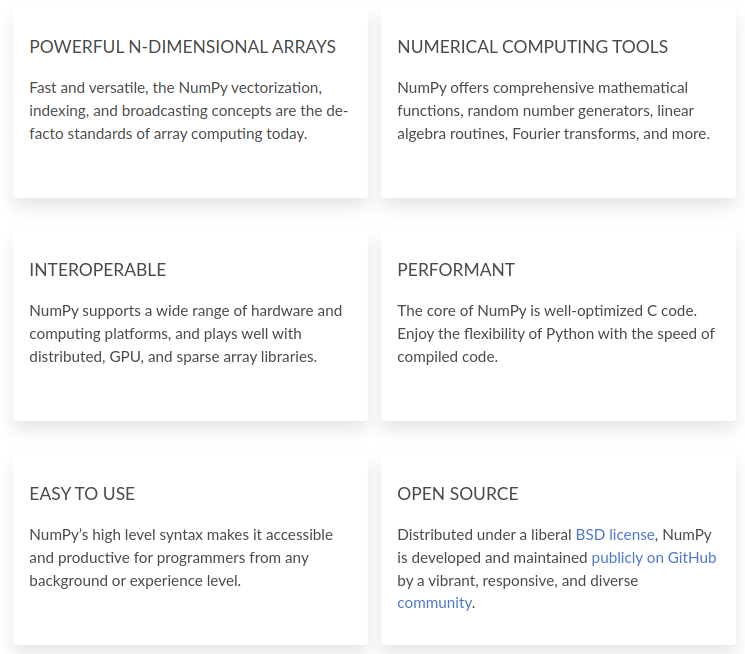
\includegraphics[width=0.75\textwidth]{../figures/numpy_overview.png}
		\end{center}
		\begin{flushright}
			\tiny{\emph{\url{numpy.org}}}
		\end{flushright}
\end{frame}

\begin{frame}
	\frametitle{NumPy Ecosystem}
		\vspace{-0.25cm}
		\begin{center}
			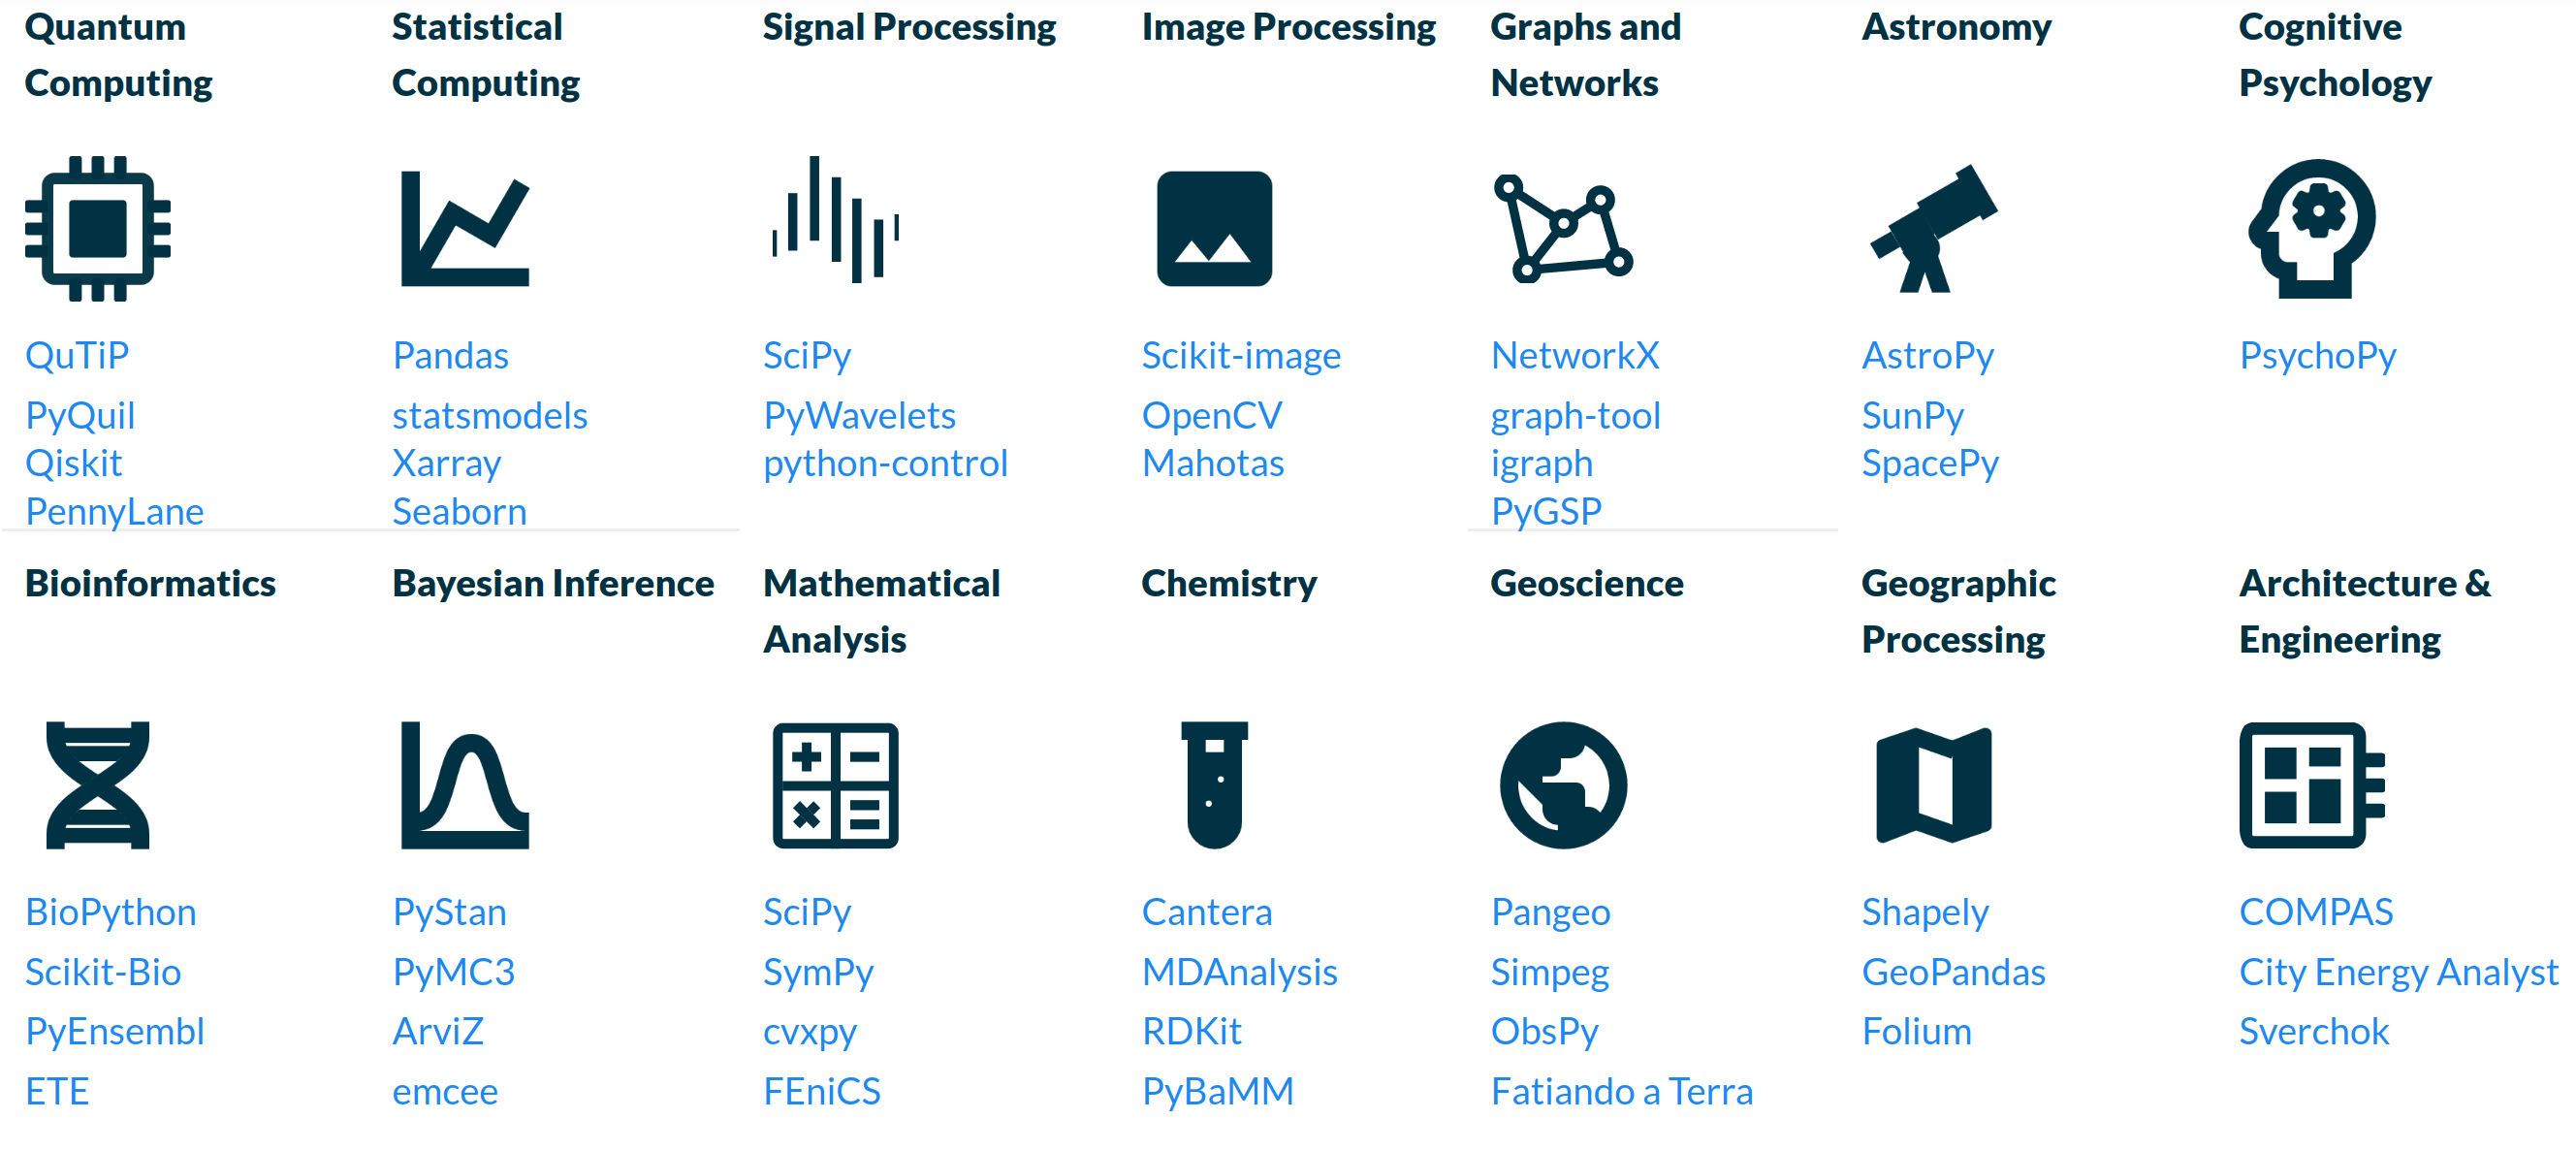
\includegraphics[width=\textwidth]{../figures/numpy_ecosystem.png}
		\end{center}
		\begin{flushright}
			\tiny{\emph{\url{numpy.org}}}
		\end{flushright}
\end{frame}

\begin{frame}
	\frametitle{NumPy Array Programming}
	\begin{itemize}
		\item Array Programming: captures the operations on arrays / matrices in intuitive syntax (closely related to the math that's trying to be expressed)
		\item Instead of looping over arrays to perform operations, NumPy efficiently implements the fundamental operations internally
		\item Results in concise, easy to-read code
		\item Reduces bugs, enhances reproducibility
	\end{itemize}

\end{frame}

\begin{frame}
	\frametitle{NumPy Array Programming}
	\begin{block}{}
	{\tiny
	 \lstinputlisting[language=python, numbers=none]{../listings/np_array_example.py}
	}
	\end{block}

	\begin{block}{}
	{\tiny
	 \lstinputlisting[language=bash, numbers=none]{../listings/np_array_example.txt}
	}
	\end{block}

	ORDERS OF MAGNITUDE DIFFERENCE!
\end{frame}

\begin{frame}
	\frametitle{NumPy Basics}
	\begin{columns}[t]
	\column{0.65\textwidth}
	\begin{block}{}
	{\tiny
	 \lstinputlisting[language=python, numbers=none]{../listings/np_basics.py}
	}
	\end{block}
	\column{0.3\textwidth}
	\begin{block}{}
	{\tiny
	 \lstinputlisting[language=bash, numbers=none]{../listings/np_basics.txt}
	}
	\end{block}
	\end{columns}

\end{frame}

\begin{frame}
	\frametitle{NumPy Basic Matrix}
	\begin{columns}[t]
	\column{0.55\textwidth}
	\begin{block}{}
	{\tiny
	 \lstinputlisting[language=python, numbers=none]{../listings/np_basics_matrix.py}
	}
	\end{block}
	\column{0.3\textwidth}
		\uncover<2->{
			\begin{center}
				\includegraphics[width=\textwidth]{../listings/face.png}\\
				Output
			\end{center}
		}
	\end{columns}

\end{frame}

\begin{frame}
	\frametitle{PLAY!}
	\begin{center}
		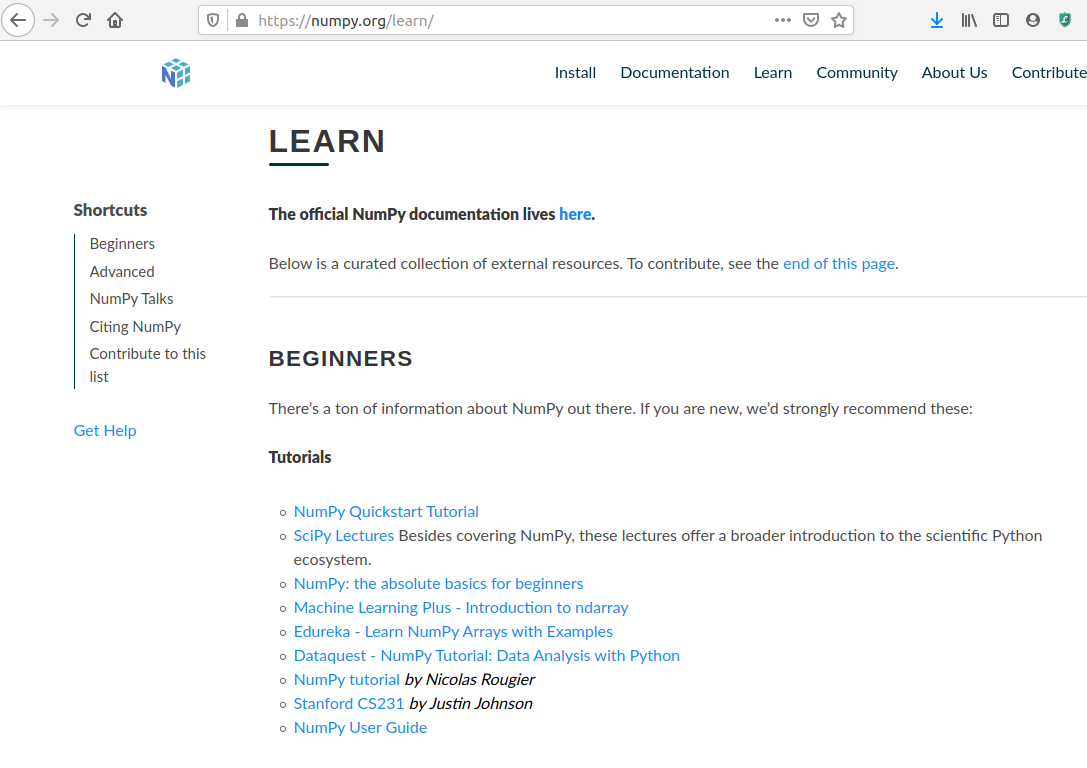
\includegraphics[width=\textwidth]{../figures/numpy_website.png}
	\end{center}
\end{frame}

\begin{frame}
	\frametitle{Pandas}
	{\bf Mission (from https://pandas.pydata.org)}
	\begin{center}
	\emph{pandas aims to be the fundamental high-level building block 
		for doing practical, real world data analysis in Python. Additionally, 
		it has the broader goal of becoming the most powerful and flexible open
		source data analysis / manipulation tool available in any language.}
	\end{center}
\end{frame}

\begin{frame}
	\frametitle{Pandas Data Structures}
	\begin{itemize}
		\item {\tt Series} - one-dimensional labeled array holding any data type
		\item {\tt DataFrame} - two-dimensional labeled data structure with columns of potentially different types (think spreadsheet), most commonly used pandas data type
	\end{itemize}
\end{frame}

\begin{frame}
	\frametitle{Pandas Data Structures}
	\begin{columns}[t]
	\column{0.5\textwidth}
	\begin{block}{}
	{\tiny
	 \lstinputlisting[language=python, numbers=none]{../listings/pandas_basics.py}
	}
	\end{block}
	\column{0.48\textwidth}
	\uncover<2->{
	\begin{block}{}
	{\tiny
	 \lstinputlisting[language=bash, numbers=none]{../listings/pandas_basics.txt}
	}
	\end{block}
	}
	\end{columns}
\end{frame}

\begin{frame}
	\frametitle{Pandas Data Frame and Time}
	\begin{columns}[t]
	\column{0.5\textwidth}
	\begin{block}{}
	{\tiny
	 \lstinputlisting[language=python, numbers=none]{../listings/pandas_timeseries.py}
	}
	\end{block}
	\column{0.48\textwidth}
	\uncover<2->{
	\begin{block}{}
	{\tiny
	 \lstinputlisting[language=bash, numbers=none]{../listings/pandas_timeseries.txt}
	}
	\end{block}
	}
	\end{columns}
\end{frame}

\begin{frame}
	\frametitle{PLAY!}
	\begin{center}
		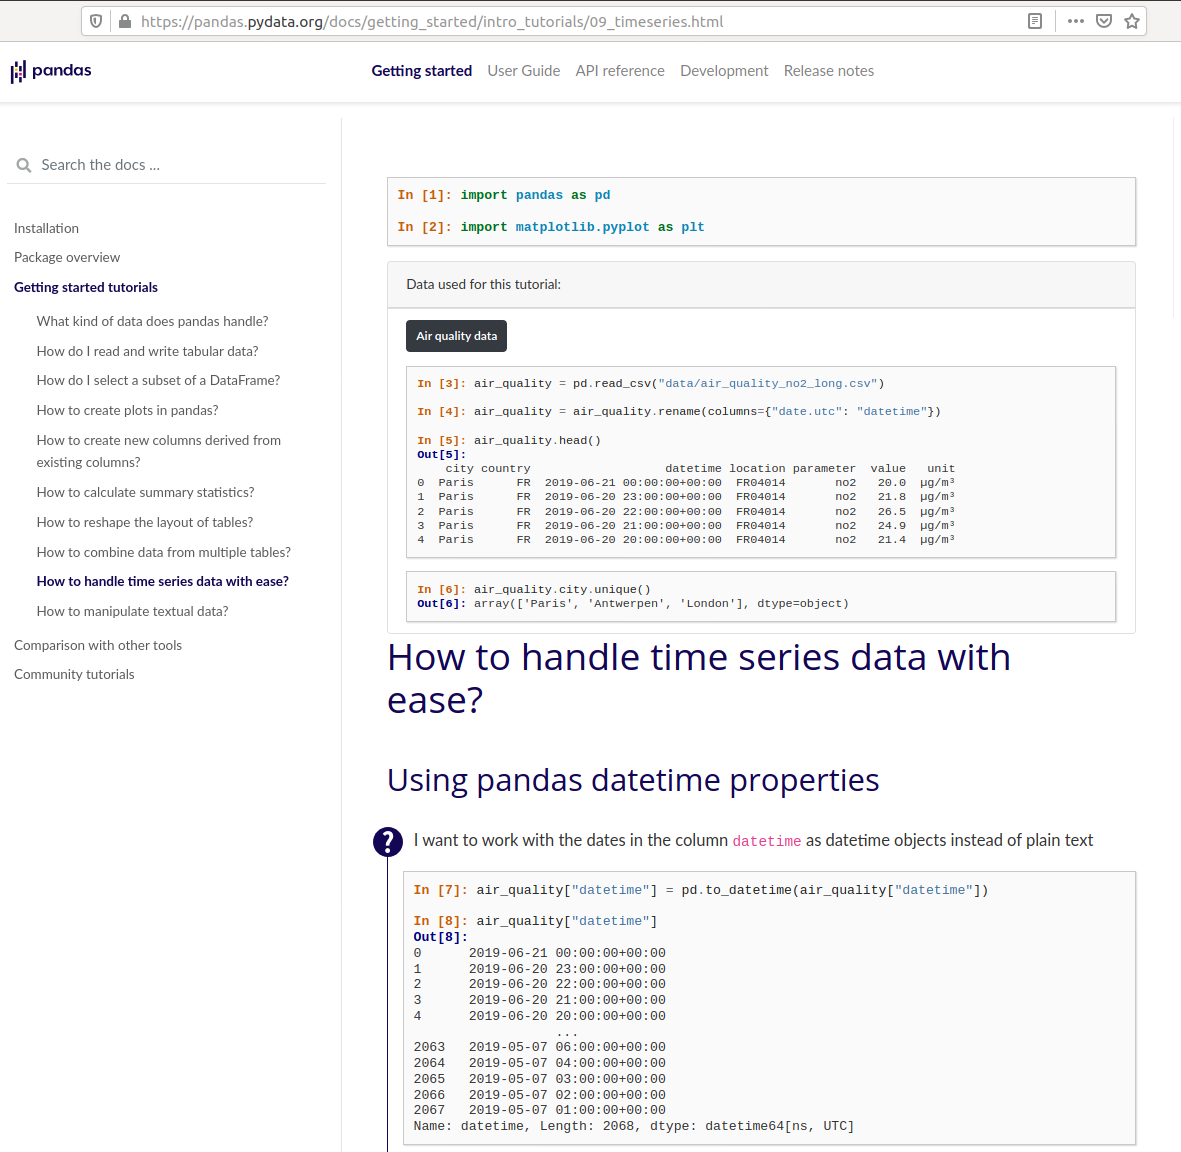
\includegraphics[width=\textwidth]{../figures/pandas_tutorials.png}
	\end{center}
\end{frame}

\end{document}
